\UC{Registrazione}

\begin{figure}[H]
    \centering
    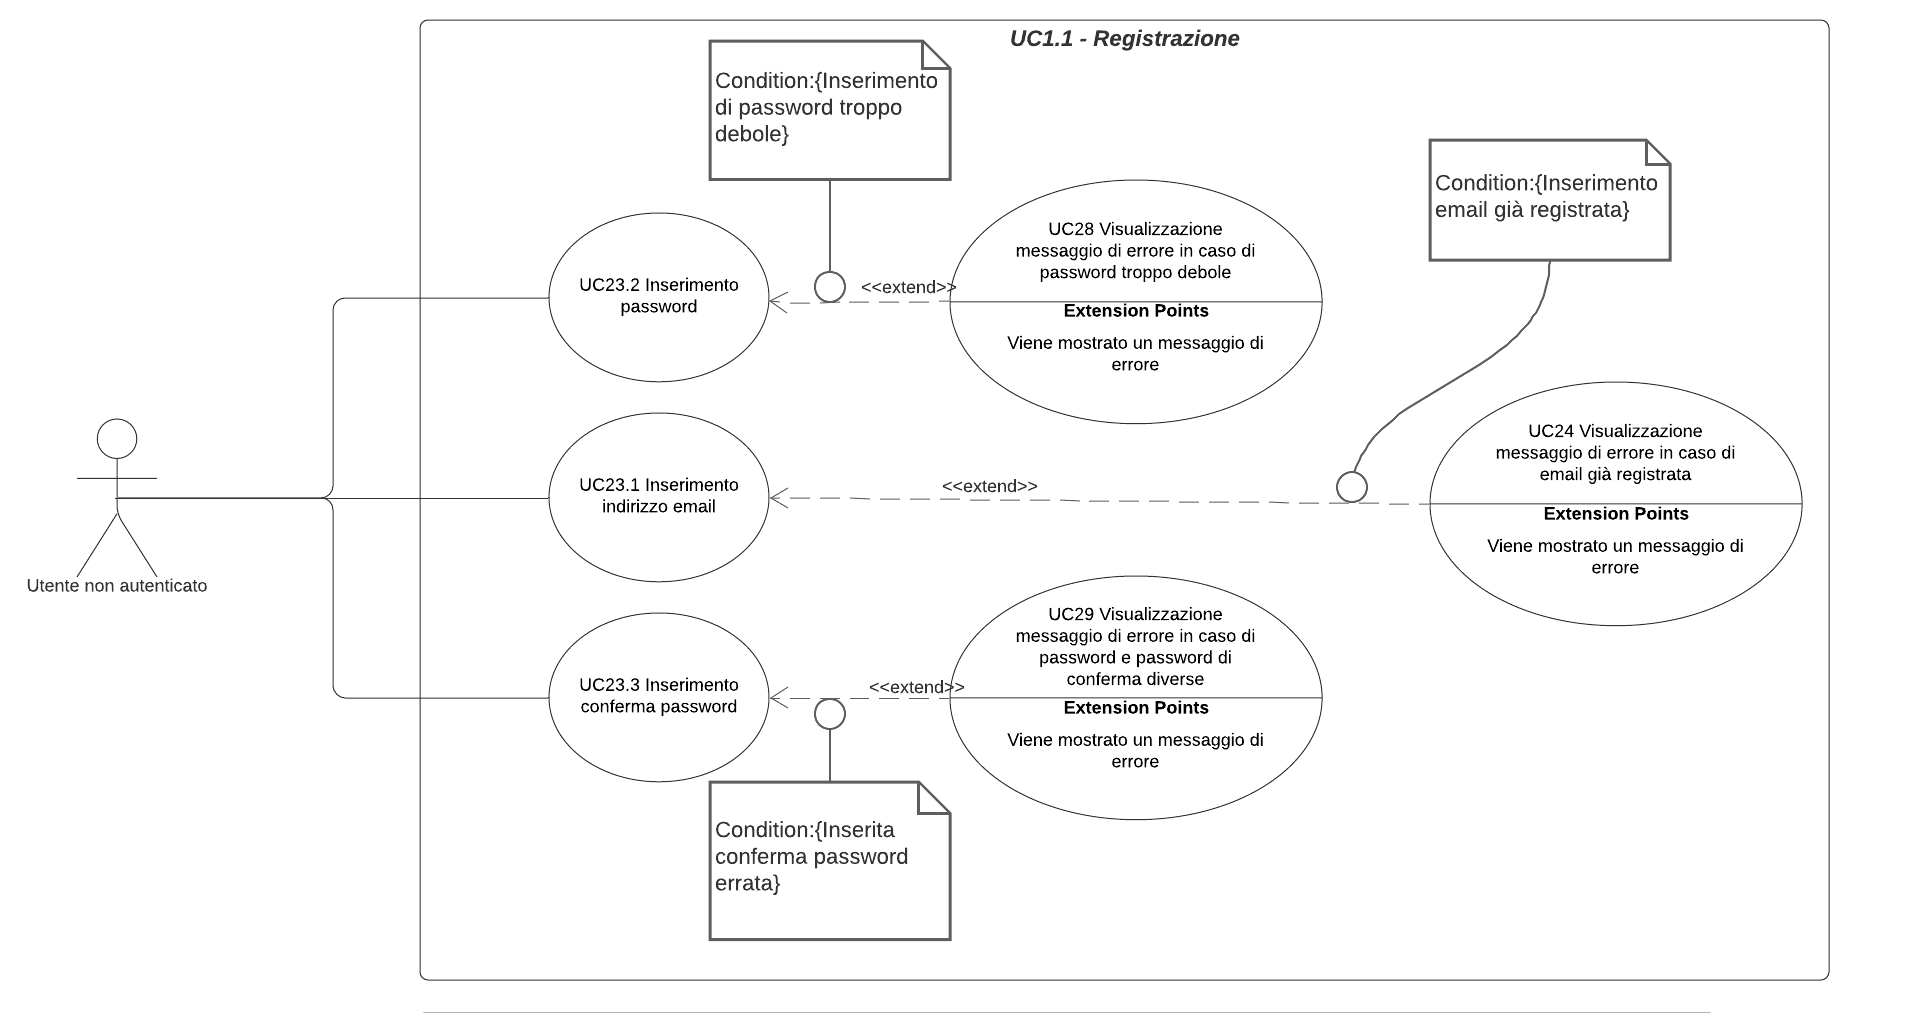
\includegraphics[scale=0.6]{Immagini/DiagrammiUC/UC1.1Registrazione}
    \caption{Diagramma di \actualUC: Registrazione}
    \label{fig:Registrazione}
\end{figure}

L'utente non autenticato che non dispone di credenziali può registrarsi e accedere come acquirente nella piattaforma usando l'email e la password.
\begin{itemize}
    \item \textbf{Attori Primari:} Utente non autenticato.
    \item \textbf{Precondizione:} L'utente non è ancora presente nella piattaforma e si trova nella pagina di registrazione.
    \item \textbf{Postcondizione:} L'utente è registrato con un account acquirente ed è autenticato come tale sulla piattaforma.
    \item \textbf{Scenario Principale:} L'utente crea un account compilando tutti i campi del modulo di registrazione nel seguente modo:
    \begin{itemize}
        \item (UC23.1) - Inserimento indirizzo e-mail.
        \item (UC23.2) - Inserimento password.
        \item (UC23.3) - Inserimento conferma password.
    \end{itemize}
    \item \textbf{Estensioni:}
    \begin{itemize}
        \item (UC24) - Visualizzazione messaggio di errore in caso di email già registrata nella piattaforma.
        \item (UC28) - Visualizzazione messaggio di errore in caso di password troppo debole. 
        \item (UC29) - Visualizzazione messaggio di errore in caso di password e password di conferma diverse. 
    \end{itemize}
\end{itemize}

\UC{Autenticazione nella piattaforma con credenziali venditore}

\begin{figure}[H]
    \centering
    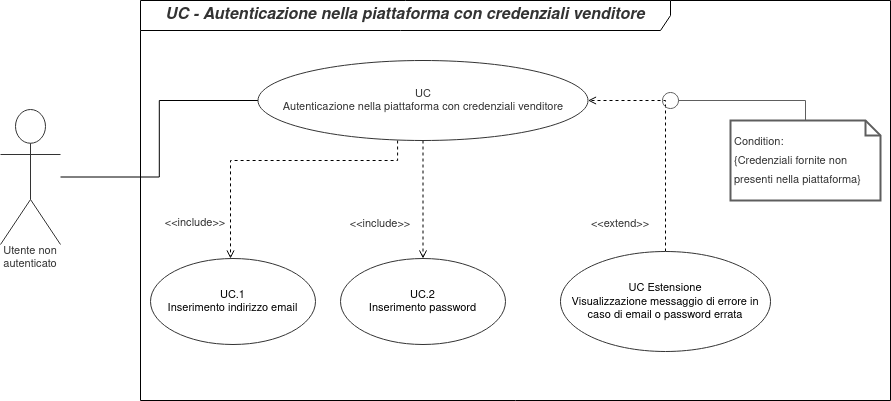
\includegraphics[scale=0.6]{Immagini/DiagrammiUC/AccessoVenditore.png}
    \caption{Diagramma di \actualUC: Autenticazione nella piattaforma con credenziali venditore} 
    \label{fig:Login}
\end{figure}

L'utente non autenticato che dispone di credenziali venditore può accedere nella piattaforma usando l'email e la password.
\begin{itemize}
    \item \textbf{Attori Primari:} Utente non autenticato.
    \item \textbf{Precondizione:} L'utente dispone di credenziali venditore e si trova nella pagina di login.
    \item \textbf{Postcondizione:} L'utente è autenticato come venditore e si trova sulla dashboard.
    \item \textbf{Scenario Principale:} L'utente accede alla piattaforma con delle credenziali in questo modo:
    \begin{itemize}
        \item (\actualUC.1) - Inserimento indirizzo.
        \item (\actualUC.2) - Inserimento password.
        \item Richiede l'autenticazione.
        \item L'utente è autenticato come venditore.
        \item L'utente viene portato alla dashboard.
    \end{itemize}
	\item \textbf{Scenario Alternativo:} L'utente compila i campi dati con delle credenziali 
	\begin{itemize}
		\item (\actualUC.1) - Inserimento indirizzo email.
		\item (\actualUC.2) - Inserimento password.
        \item Richiede l'autenticazione.
    \end{itemize}
	Ma le credenziali fornite non appartengono alla piattaforma, quindi:
	\begin{itemize}
		\item Viene visualizzato un messaggio di errore apposito (UC estensione)
		\item L'utente rimane non autenticato e alla pagina di login.
	\end{itemize}
    \item \textbf{Estensioni:}
    \begin{itemize}
        \item (UC) - Visualizzazione messaggio di errore in caso di email o password errata.
    \end{itemize}
    \item \textbf{Inclusioni:}
    \begin{itemize}
    	\item \actualUC.1 - Inserimento indirizzo email.
    	\item \actualUC.2 - Inserimento password. 
    \end{itemize}
\end{itemize}

\resetSubUC
\subUC{Inserimento indirizzo email}
\begin{itemize}
	\item \textbf{Attori Primari:} Utente non autenticato.
	\item \textbf{Precondizione:} L'utente non è autenticato
	\item \textbf{Postcondizione:} L'utente ha inserito il proprio indirizzo email.
	\item \textbf{Scenario Principale:} Inserimento email per l'autenticazione.
	\item \textbf{Scenario Secondario:} L'utente non inserisce l'email:
	\begin{itemize}
		\item (UC ) - Viene mostrato un messaggio d'errore.
		\item L'utente non può procedere all'autenticazione.
	\end{itemize}
	\item \textbf{Estensioni:}
	\begin{itemize}
		\item \item (UC) - Visualizzazione messaggio campo dati obbligatorio non inserito.
	\end{itemize}
\end{itemize}

\subUC{Inserimento password}
\begin{itemize}
	\item \textbf{Attori Primari:} Utente non autenticato.
	\item \textbf{Precondizione:} L'utente non è autenticato
	\item \textbf{Postcondizione:} L'utente ha inserito la propria password.
	\item \textbf{Scenario Principale:} inserimento password per l'autenticazione.
		\item \textbf{Scenario Secondario:} L'utente non inserisce la password:
	\begin{itemize}
		\item (UC ) - Viene mostrato un messaggio d'errore.
		\item L'utente non può procedere all'autenticazione.
	\end{itemize}
	\item \textbf{Estensioni:}
	\begin{itemize}
		\item \item (UC) - Visualizzazione messaggio campo dati obbligatorio non inserito.
	\end{itemize}
\end{itemize}

\UC{Autenticazione nella piattaforma con credenziali acquirente}

\begin{figure}[H]
	\centering
	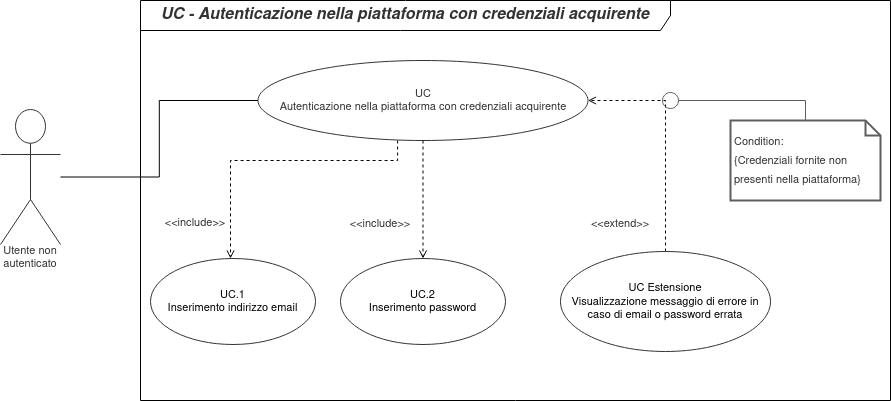
\includegraphics[scale=0.6]{Immagini/DiagrammiUC/AccessoAcquirente.png}
	\caption{Diagramma di \actualUC: Autenticazione nella piattaforma con credenziali acquirente} 
	\label{fig:Login}
\end{figure}

L'utente non autenticato che dispone di credenziali acquirente può accedere nella piattaforma usando l'email e la password.
\begin{itemize}
	\item \textbf{Attori Primari:} Utente non autenticato.
	\item \textbf{Precondizione:} L'utente dispone di credenziali acquirente e si trova nella pagina di login.
	\item \textbf{Postcondizione:} L'utente è autenticato come acquirente e si trova nella pagina di provenienza.
	\item \textbf{Scenario Principale:} L'utente accede alla piattaforma con delle credenziali in questo modo:
	\begin{itemize}
		\item (\actualUC.1) - Inserimento indirizzo email venditore.
		\item (\actualUC.2) - Inserimento password.
		\item Richiede l'autenticazione.
		\item L'utente è autenticato come acquirente.
		\item L'utente viene portato alla pagina da cui proveniva prima del login.
	\end{itemize}
	\item \textbf{Scenario Alternativo:} L'utente compila i campi dati con delle credenziali 
	\begin{itemize}
		\item (\actualUC.1) - Inserimento indirizzo.
		\item (\actualUC.2) - Inserimento password.
		\item Richiede l'autenticazione.
	\end{itemize}
	Ma le credenziali fornite non appartengono alla piattaforma, quindi:
	\begin{itemize}
		\item Viene visualizzato un messaggio di errore apposito (UC estensione)
		\item L'utente rimane non autenticato e alla pagina di login.
	\end{itemize}
	\item \textbf{Estensioni:}
	\begin{itemize}
		\item (UC) - Visualizzazione messaggio di errore in caso di email o password errata.
	\end{itemize}
	\item \textbf{Inclusioni:}
	\begin{itemize}
		\item \actualUC.1 - Inserimento indirizzo email.
		\item \actualUC.2 - Inserimento  password. 
		\end{itemize}
\end{itemize}

\resetSubUC
\subUC{Inserimento indirizzo email}
\begin{itemize}
	\item \textbf{Attori Primari:} Utente non autenticato.
	\item \textbf{Precondizione:} L'utente non è autenticato
	\item \textbf{Postcondizione:} L'utente ha inserito il proprio indirizzo email.
	\item \textbf{Scenario Principale:} Inserimento email per l'autenticazione.
	\item \textbf{Scenario Secondario:} L'utente non inserisce l'email:
	\begin{itemize}
		\item (UC ) - Viene mostrato un messaggio d'errore.
		\item L'utente non può procedere all'autenticazione.
	\end{itemize}
	\item \textbf{Estensioni:}
	\begin{itemize}
		\item \item (UC) - Visualizzazione messaggio campo dati obbligatorio non inserito.
	\end{itemize}
\end{itemize}

\subUC{Inserimento password}
\begin{itemize}
	\item \textbf{Attori Primari:} Utente non autenticato.
	\item \textbf{Precondizione:} L'utente non è autenticato
	\item \textbf{Postcondizione:} L'utente ha inserito la propria password.
	\item \textbf{Scenario Principale:} inserimento password per l'autenticazione.
	\item \textbf{Scenario Secondario:} L'utente non inserisce la password:
	\begin{itemize}
		\item (UC ) - Viene mostrato un messaggio d'errore.
		\item L'utente non può procedere all'autenticazione.
	\end{itemize}
	\item \textbf{Estensioni:}
	\begin{itemize}
		\item \item (UC) - Visualizzazione messaggio campo dati obbligatorio non inserito.
	\end{itemize}
\end{itemize}

\UC{Password dimenticata}

\begin{figure}[H]
    \centering
    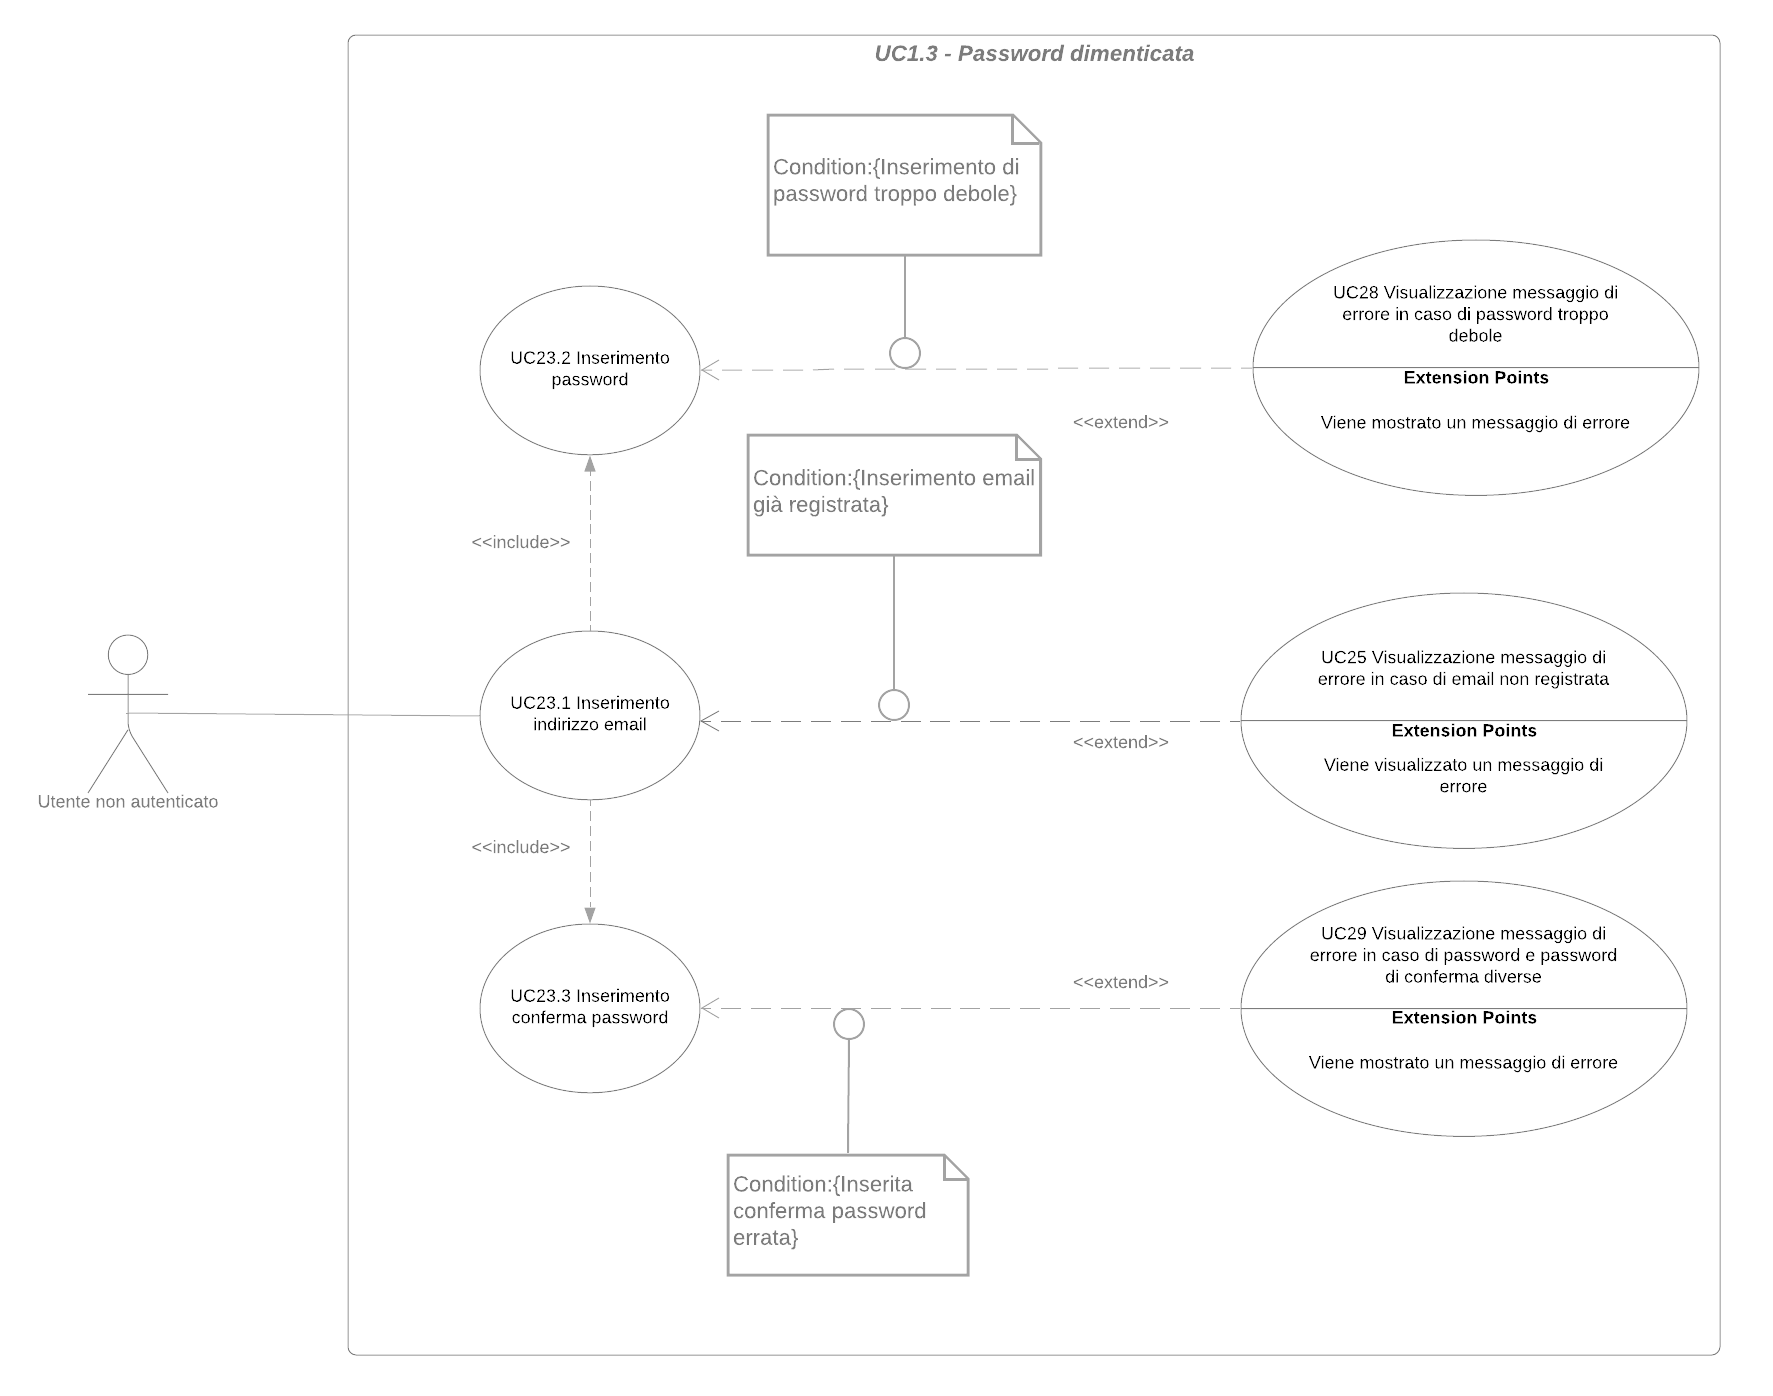
\includegraphics[scale=0.2]{Immagini/DiagrammiUC/UC1.3PasswordDimenticata.png}
    \caption{Diagramma di \actualUC: Password dimenticata} 
    \label{fig:PasswordDimenticata}
\end{figure}

L'utente che dispone di credenziali si è dimenticato la propria password e la vuole cambiare.
\begin{itemize}
    \item \textbf{Attori Primari:} Utente non autenticato.
    \item \textbf{Precondizione:} L'utente non autenticato che dispone di credenziali si trova nella pagina per cambiare la password.
    \item \textbf{Postcondizione:} L'utente è autenticato e ha cambiato la password con cui accedere.
    \item \textbf{Scenario Principale:} L'utente che dispone di credenziali si è dimenticato la propria password e per cambiarla deve compiere i seguenti passi:
    \begin{itemize}
        \item Andare nella pagina di cambiamento password. 
        \item (UC23.1) - Inserimento email.
        \item Invio link per il cambio della password all'email indicata.
        \item Apertura della pagina per il cambio della password.
        \item (UC23.2) - Inserimento nuova password.
        \item (UC23.3) - Inserimento conferma nuova password.
        \item L'utente è autenticato e ha cambiato la password.
    \end{itemize}
    \item \textbf{Estensioni:}
    \begin{itemize}
        \item (UC25) - Visualizzazione messaggio di errore in caso di email non registrata.
        \item (UC28) - Visualizzazione messaggio di errore in caso di password troppo debole. 
        \item (UC29) - Visualizzazione messaggio di errore in caso di password e password di conferma diverse. 
    \end{itemize}
    \item \textbf{Inclusioni:}
    \begin{itemize}
        \item (UC23.2) - Inserimento nuova password.
        \item (UC23.3) - Inserimento conferma nuova password.
    \end{itemize}
\end{itemize}

\UC{Logout dalla piattaforma}
L'utente autenticato decide di scollegarsi dalla piattaforma.
\begin{itemize}
    \item \textbf{Attori Primari:} Utente autenticato.
    \item \textbf{\glo{Precondizione}:} L'utente è autenticato e preme sull'azione di scollegamento.
    \item \textbf{\glo{Postcondizione}:} L'utente autenticato diventa un utente non autenticato.
    \item \textbf{Scenario Principale:} L'utente autenticato decide di scollegarsi dalla piattaforma e preme sull'azione di scollegamento.
\end{itemize}
